\documentclass{article}

\usepackage{graphicx}
\usepackage{cleveref}
\usepackage{listings}
\usepackage{booktabs}

\usepackage[vmargin=2.2cm]{geometry}

\usepackage[T1]{fontenc}
\usepackage[utf8]{inputenc}
\usepackage{helvet}
\renewcommand{\familydefault}{\sfdefault}

\usepackage{harvard}
\usepackage{bibgerm}

\title{Pfad Plannung A* vs ROS nativ}
\date{2020 Juni}
\author{Jonathan König}

\begin{document}

\maketitle
\newpage

\tableofcontents

\newpage
\clearpage
\pagenumbering{arabic}



\section{Aufgabenstellung}

\begin{figure}[!htbp]
    \centering
    
\includegraphics[width=0.5\linewidth]{../src/koenig/maps/bmrMap.png}
    \caption{Maze}\label{map}
\end{figure}

Es sollte eine Pfad durch das Labyrinnt, siehe Abbildung \ref{map}, geplannt werden.
gestarted sollte am unteren Eingang und der Ausgang sollte der linkere obere sein.

Es sollten zwei Lösungen implementiert werden:
\begin{enumerate}
    \item mithilfe eines von ROS bereits vorhanden Pfad planner einen Pfad erstellen lassen
    \item Selber einen Pfad plannungs Algorythmus schreiben 
\end{enumerate}

\section{ROS DWAPlannerROS}
\label{DWAPlannerROS}

Das Ziel wird über eine eigens geschrieberne Node \verb|goal_pub| über einen Action Client an die \verb|move_base| Node übergeben.
Die Node \verb|move_base| holt sich über die Nodes \verb|joint_state_publisher| und \verb|robot_state_publisher| die Daten zum turtlebot burger.
über die Node tf wird dann der Roboter in eine Startposition verschoben.



\verb|move_base| published dann einen Pfad, siehe Abbildung \ref{path_nativ}.

\begin{figure}[!htbp]
    \centering
    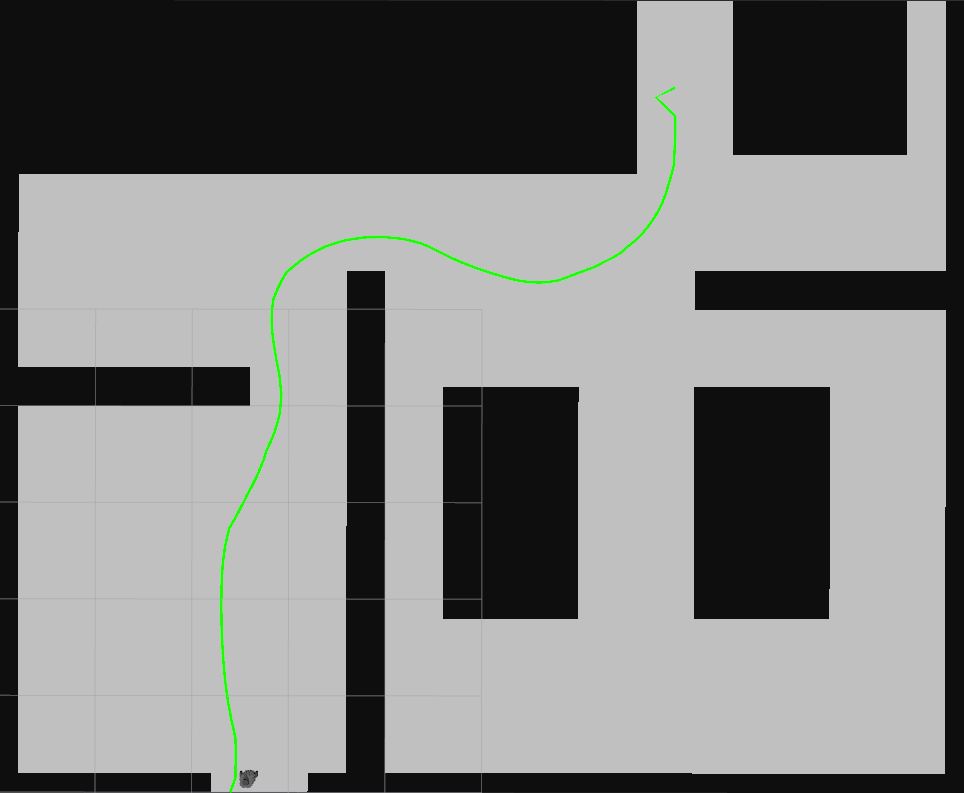
\includegraphics[width=0.5\linewidth]{PICs/nativ_rviz_plan.png}
    \caption{Native Pfad}\label{path_nativ}
\end{figure}

\section{Custom Path Planner}

Um selber einen Pfad plannen zu können wurde die Node \verb|finder| geschrieben.
Um die Node \verb|goal_pub| weiter verwenden zu können ist in den Node \verb|finder| ein Action Server intergriert um die Node \verb|goal_pub| weiter verwenden zu können.

Implementiert wurde der A Star Algorythmus.\newline

Dafür wurde eine Klasse \texttt{pixel} erstellt welche Attribute für jedes Raster Teil der Karte beinhaltet.

\begin{lstlisting}
class pixel{
    public:
        bool is_obstical;
        pair<int, int> parents, location;
        double goal_distance;
        double walked_distance, heuristik;

        pixel();
};
\end{lstlisting}

Bevor begonnen wir zu suchen wir für jeden pixel die \verb|location| und die \verb|goal_distance| gesetzt. 
Daraufhin wird der A Start Algorythmus für die Start und Ziel position durchgeführt und der Pfad gepublished, siehe \ref{path_custom}.

\begin{figure}[!htbp]
    \centering
    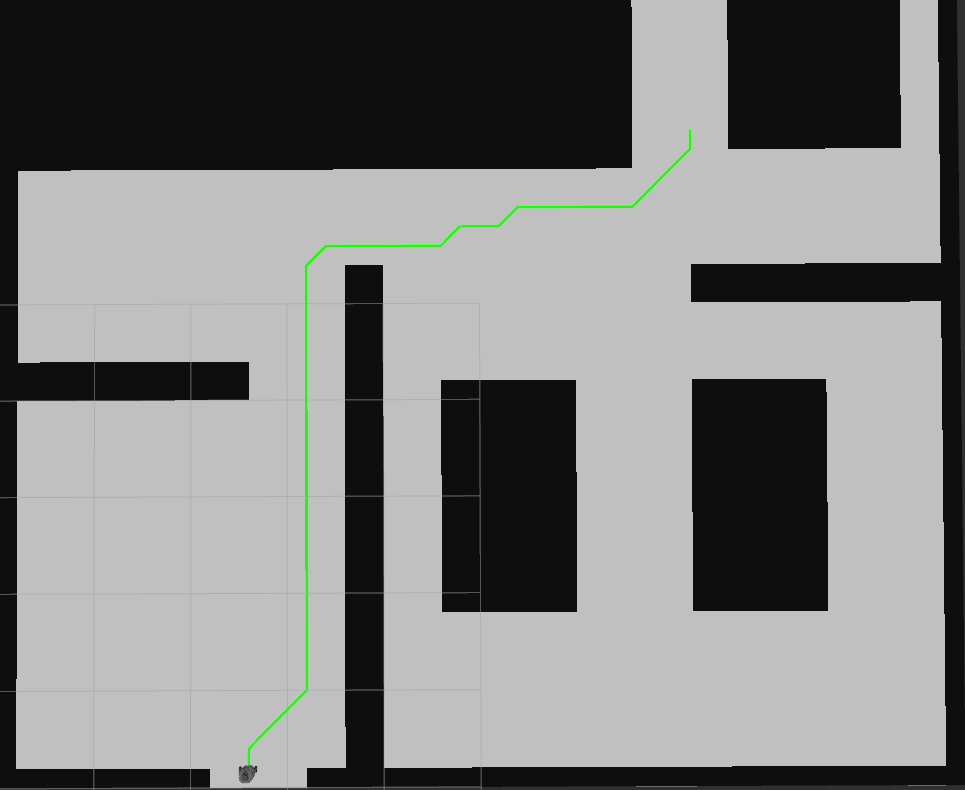
\includegraphics[width=0.5\linewidth]{PICs/custom_rviz_plan.png}
    \caption{Custom Pfad}\label{path_custom}
\end{figure}

\section{Vegleich der beiden Lösungen}

\textbf{Completeness}\newline

\begin{table}[!htbp]
    \begin{tabular}{p{7cm}|p{7cm}}
        DWAPlannerROS & custom A Star \\ \bottomrule
        Lösung vorhanedn & Lösung vorhanedn
    \end{tabular}
\end{table}

\textbf{Optimality}\newline

\begin{table}[!htbp]
    \begin{tabular}{p{7cm}|p{7cm}}
        DWAPlannerROS & custom A Star \\ \bottomrule
     berücksichtigt das der Roboter nicht unendlich schnell sich drehen kann & Sollte den kürzesten Pfad finden doch nur mit 45 pfaden möglich
    \end{tabular}
\end{table}


\textbf{Time complexity}\newline

\begin{table}[!htbp]
    \begin{tabular}{p{7cm}|p{7cm}}
        DWAPlannerROS & custom A Star \\ \bottomrule
    langsamer & schneller als Dikstra weil weniger Knoten durchsucht werden müssen aufgrund der Heristik
    \end{tabular}
\end{table}

\textbf{Space complexity}\newline

\begin{table}[!htbp]
    \begin{tabular}{p{7cm}|p{7cm}}
        DWAPlannerROS & custom A Star \\ \bottomrule
        test & some
    \end{tabular}
\end{table}


\end{document}
